% Chapter 5, Results.
% Generated from Dissertation/Chapter5_Results.md by tools/md2tex.py.
%% The draft-status line, the provenance notes and the [edit] markers in the
%% Markdown source are not part of the submitted text and are absent here.
%% Markdown is the source. Regenerate this file when it changes; do not hand-edit.

\chapter{Results}
\label{ch:results}
\lhead{Chapter 5. \emph{Results}}

This chapter reports what the planning model returns on the trust's own queues. It gives the capacity ceiling and which trials reach it, tests how reliably a plan delivers what it promises, and identifies what limits the number and what raising it costs. Table~\ref{tab:analyses} maps each analysis to the sub-question it answers.

\section{The model's decision on the real queues}
\label{sec:realqueues}

The model was solved at each of the 25 decision points of Section~\ref{sec:experiments}. Figure~\ref{fig:planactual} sets its plan against what the service actually did.

\begin{figure}[htbp]
  \centering
  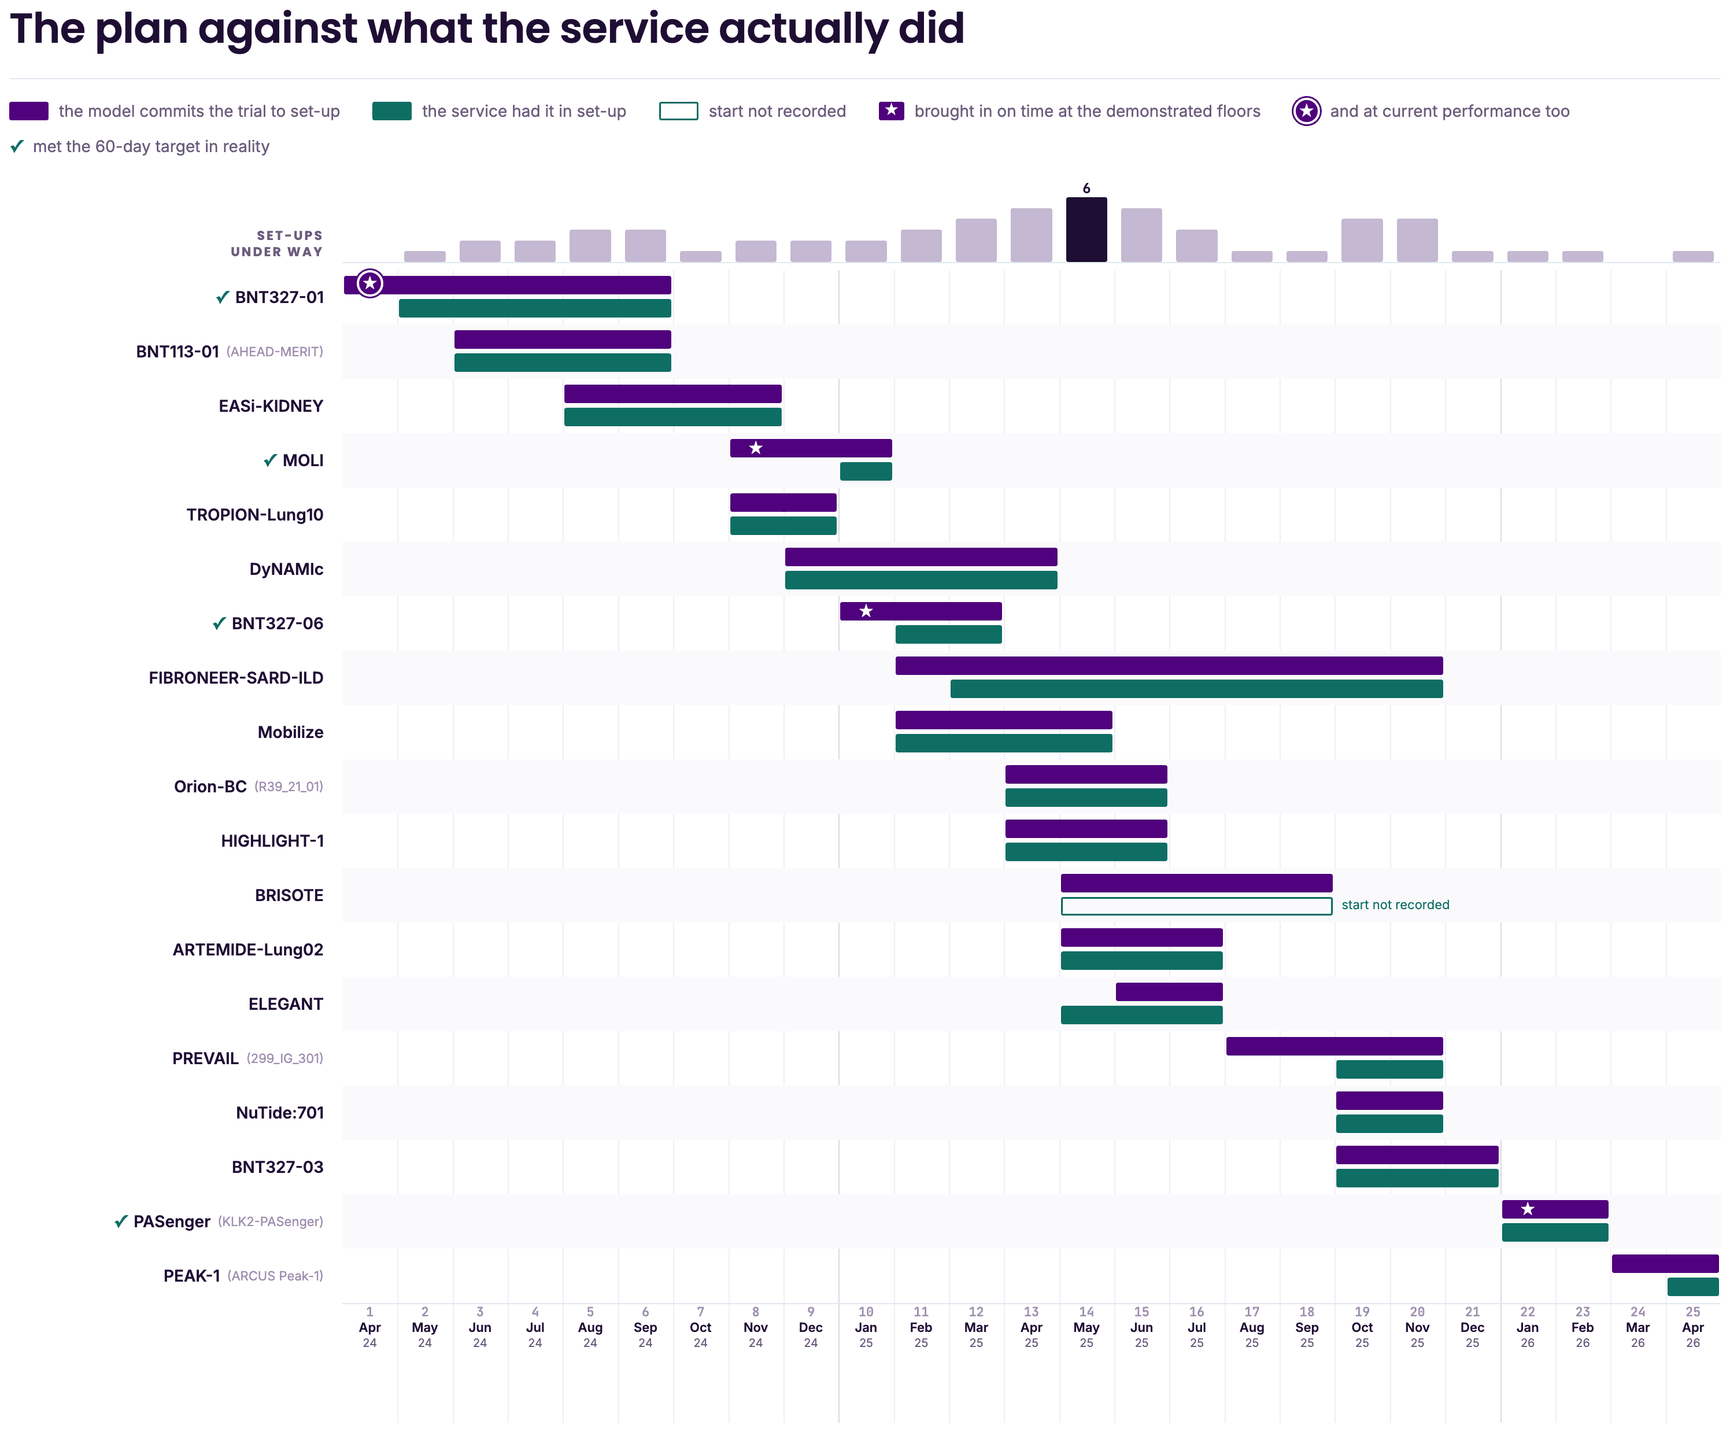
\includegraphics[width=\textwidth]{fig5_1_plan_vs_actual.png}
  \caption{The plan against what the service actually did, by month of commitment rather than by date}
  \label{fig:planactual}
\end{figure}

Only four trials ever finish on time, and they are exactly the four that met the target in reality. The model identifies these trials in advance rather than in hindsight; it does not uncover any additional trial that the service could have brought in on time.

Against the stated ``commit the longest waiter'' rule, the model performs better when capacity is limited. It brings a trial in on time in 10 of the 25 months at both one and two set-ups per month, compared with 6 and 7 months respectively for the rule. From three set-ups per month onwards, both approaches commit the same trials and perform equally.

The 10 months cover only four trials. Because the plan is remade each month, a trial that still fits is re-committed and counted again. The comparator is a stated arrival-order rule, not an observed record of practice.

A sweep of 9,000 synthetic portfolios tests whether that pattern holds beyond the trust's own queues. At current performance the model never beats the arrival-order rule for on-time completions. At the demonstrated floors it wins in 36\% of cases, each win costing 24.3 weighted days of lateness elsewhere, and it helps most when trials arrive early and the aseptic share is low. Appendix 5.A holds the design, the limitations and the full grid.

\section{Why the model picks these and not others}
\label{sec:whythese}

The model starts the right trials sooner. Three of the four trials it brings in on time are among the six it starts earliest: MOLI by 34 days, BNT327-06 by 22 days, and BNT327-01 by 17 days. Appendix 5.D sets the model's start date against the service's own for all nineteen.

The service's own head start bought little: of the twelve trials it began before the model would, eleven missed the target anyway. Waiting is what consumes the window, and the trial that can still finish is usually the one that has just arrived; Appendix 5.D works through November 2024.

Figure~\ref{fig:allcases} shows why so few can finish at all, placing the 19 studies with a computable clock start on one axis measured in days from that start.

\begin{figure}[htbp]
  \centering
  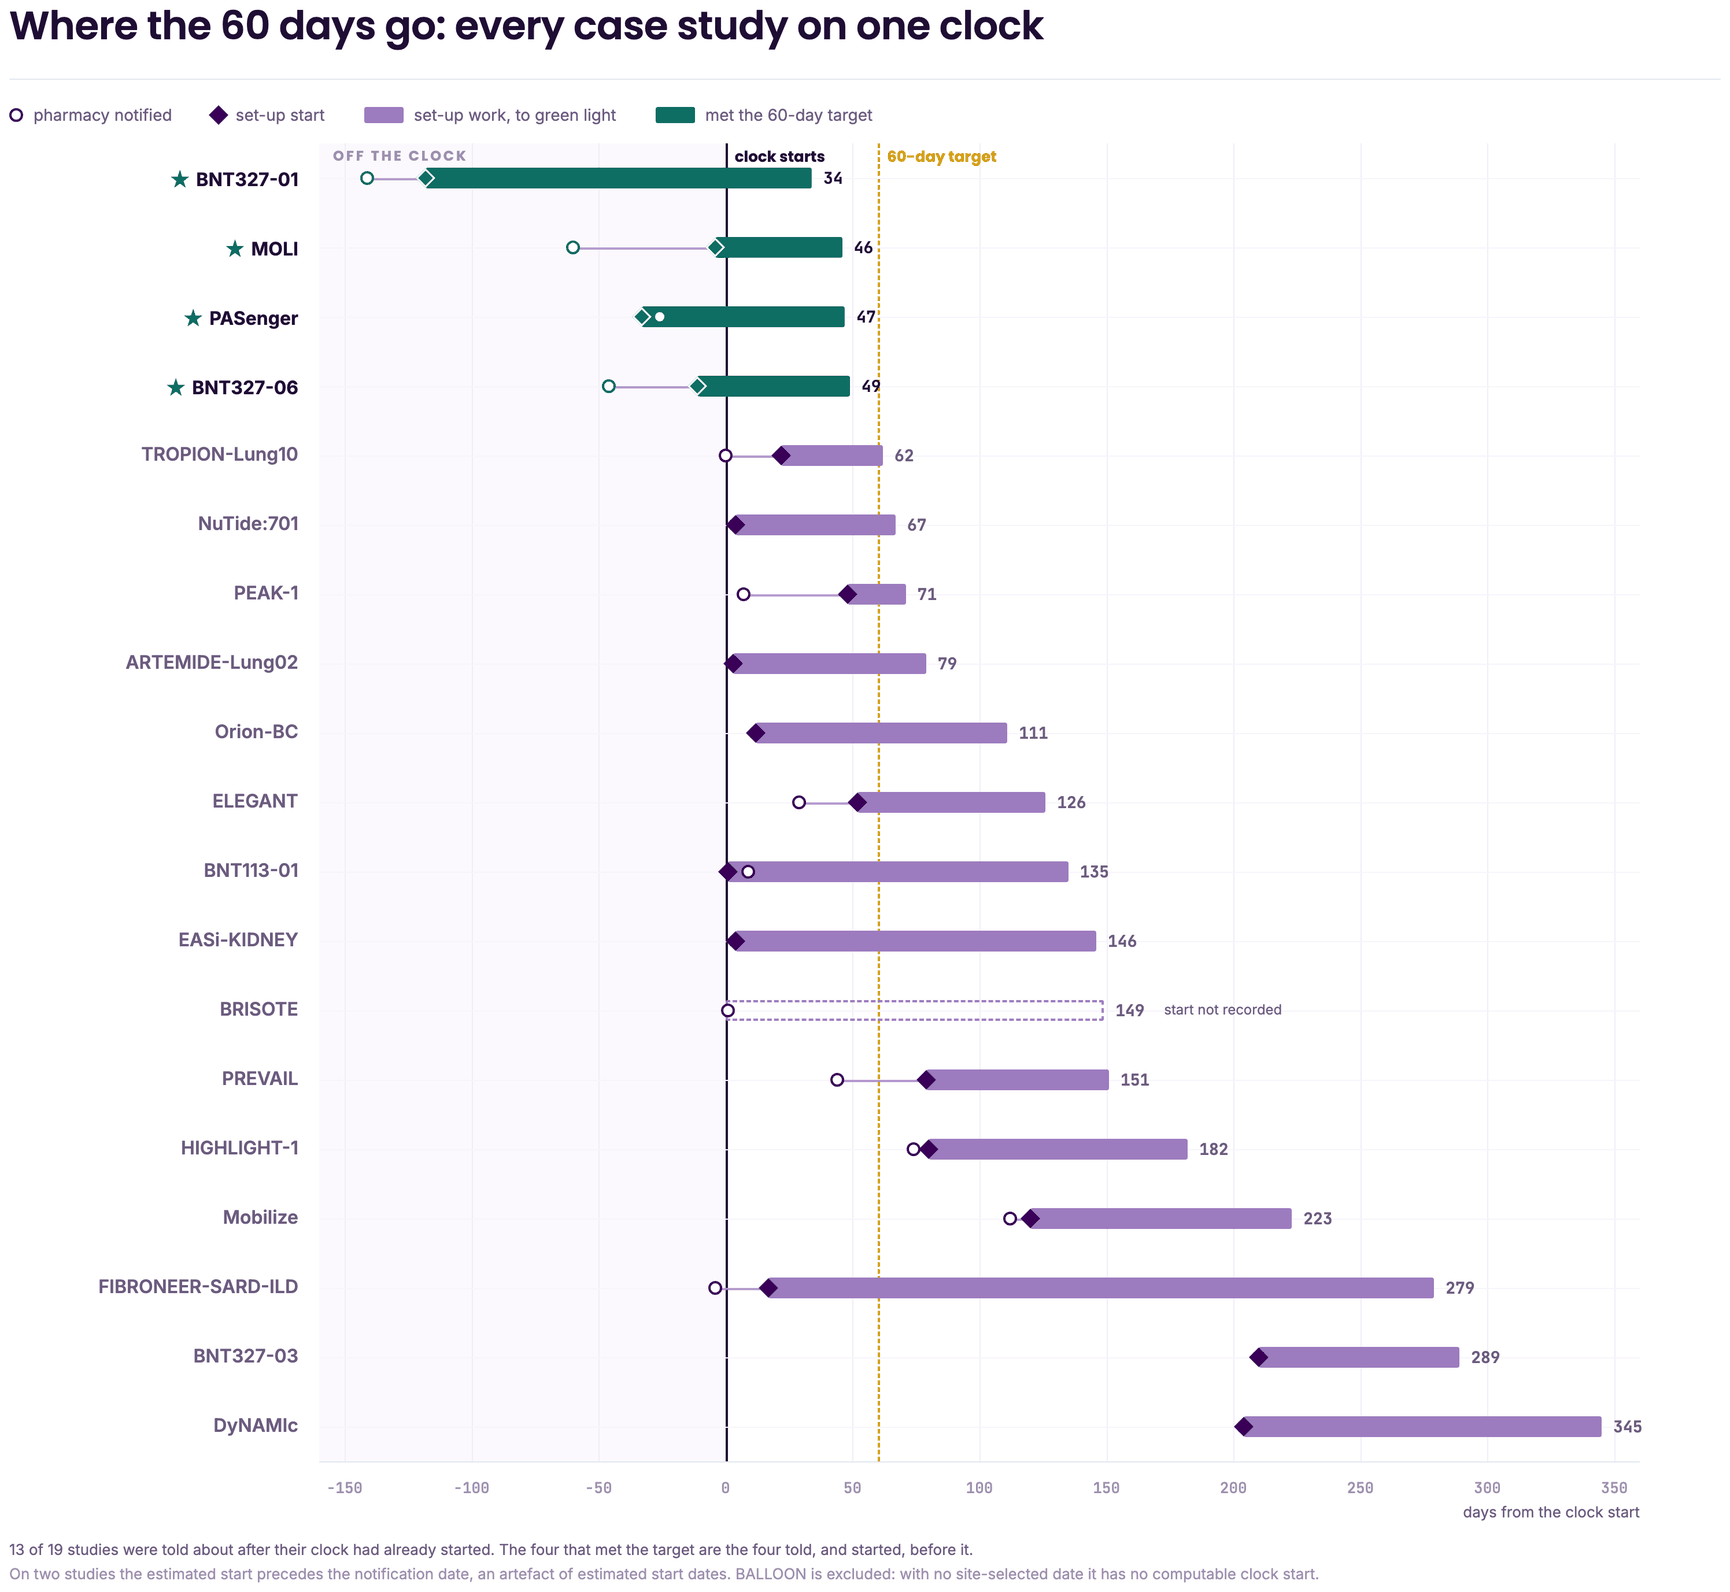
\includegraphics[width=\textwidth]{fig5_3_all_cases_timeline.png}
  \caption{Where the 60 days go: every case study on one clock}
  \label{fig:allcases}
\end{figure}

Four trials met the target, and all entered the pharmacy queue before the 60-day clock began.

\begin{table}[htbp]
  \centering
  \caption{The four trials that met the 60-day target}
  \label{tab:fourtrials5}
  \begin{tabularx}{\textwidth}{@{}lLLL@{}}
    \toprule
    \textbf{Trial} & \textbf{Days entered before clock start} & \textbf{Work interval (days)} & \textbf{Clock interval (days)} \\
    \midrule
    MOLI & 4 & 50 & 46 \\
    \addlinespace
    BNT327-06 & 11 & 60 & 49 \\
    \addlinespace
    PASenger & 33 & 80 & 47 \\
    \addlinespace
    BNT327-01 & 118 & 152 & 34 \\
    \bottomrule
  \end{tabularx}
\end{table}

Starting earlier did not shorten the work. Work intervals did not differ significantly between early and late starters ($p = 0.71$). Instead, earlier starts moved some work outside the 60-day window. Two of the four trials met the target despite requiring more than 60 days of work because their set-up began before the window opened. The window did not stretch; the work began earlier. No recorded trial characteristic predicted an early start (Appendix 4.I).

Where the plan falls short, it does so by relatively little. Four trials missed the target by 20 days or less in reality and, under the plan, fall 10 to 29 days short of their available windows. This shortfall reflects insufficient time in the window, not a failure to choose between trials. No selection rule can recover those days; Section 5.4 examines what would add them.

\section{Plan delivery under duration uncertainty}
\label{sec:delivery}

A solved plan produces one on-time count from a single planned duration for each pathway, so the uncertainty run of Section~\ref{sec:experiments} and Appendix 4.J.6.2 replays each committed plan 10,000 times to report how often that count is actually met. Appendix 5.F reports what the real February queue delivers, and Figure~\ref{fig:planuncertainty} the synthetic one.

In the real February queue, neither duration basis produced a plan promising an on-time completion. The simulation therefore describes outcome variability rather than delivery reliability for a positive promise; approval delay is held at its expected value throughout, so every reported figure understates total uncertainty. Appendix 5.F reports the distribution.

The synthetic standing queue of 16 trials described in Appendix 4.G, used in this section alone and labelled synthetic throughout, is the one that carries a promise. At current performance it promises zero and delivers zero in every one of the 10,000 runs. At the demonstrated floors it promises three, and Figure~\ref{fig:planuncertainty} shows what arrives: three in 32.6\% of runs, but two in 48.5\%. The promised three therefore lands in about a third of runs, two is the most likely single outcome, and one is the highest count reached in at least 90\% of runs.

\begin{figure}[htbp]
  \centering
  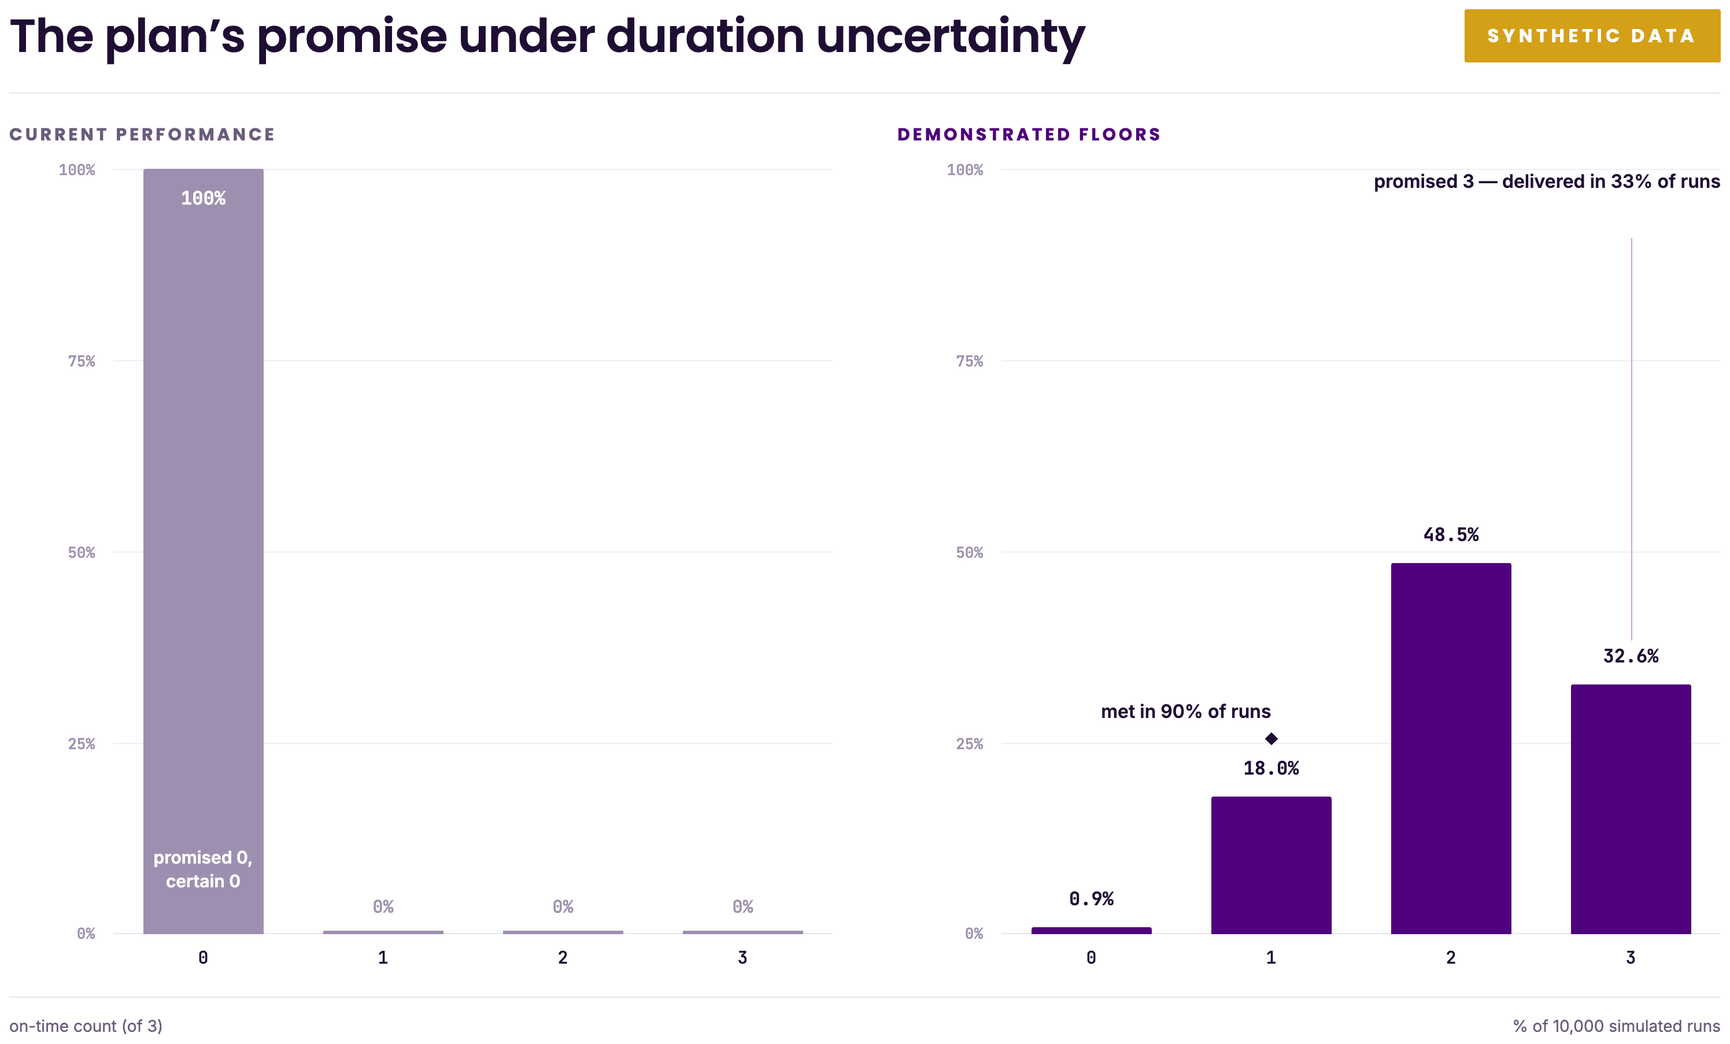
\includegraphics[width=\textwidth]{fig5_4_plan_uncertainty.png}
  \caption{The plan's promise under duration uncertainty (synthetic queue)}
  \label{fig:planuncertainty}
\end{figure}

The point is the deterministic verdict, not any single trial. Where a plan records a trial as one day late, that margin sits well inside the observed spread of set-up durations, so the label carries no information and a trivial change of input reverses it. Where the margin is smaller than the spread, the deterministic result is a tie-break rather than a finding; Appendix 5.F works through the case behind this.

\section{What would have to change}
\label{sec:levers}

Six settings could change the results. Table~\ref{tab:settings} reports what each one does, and the two columns disagree in a way that matters.

\begin{table}[htbp]
  \centering
  \caption{What each setting changes, across twenty-five decision points}
  \label{tab:settings}
  \begin{tabularx}{\textwidth}{@{}lLLLL@{}}
    \toprule
    \textbf{Setting} & \textbf{Intervention tested / observed span} & \textbf{Months $\geq$1 on time (of 25)} & \textbf{Best count} & \textbf{Largest single-date lateness reduction} \\
    \midrule
    Preparation lead, committed trials & 0, 7, 14, 21, 35, 60 days & 20 of 25 & 3 & 394 \\
    \addlinespace
    Pharmacy queue, notification to start & Return 0, 25, 50, 75 or 100\% of each trial's observed wait, which spans 0 to 23 days & 14 of 25 & 2 & 76 \\
    \addlinespace
    Hand-over gap, clock to notification & Return 0, 25, 50, 75 or 100\% of each trial's observed gap, which spans 0 to 112 days & 11 of 25 & 2 & 498 \\
    \addlinespace
    Slots opened per month & 1, 2, 3, 4, 5, 6 & 9 of 25 & 1 & 154 \\
    \addlinespace
    Hands-on days per approval & 0.5, 1.0, 2.0, 3.0 days & 9 of 25 & 1 & 20 \\
    \addlinespace
    Target window & 55, 60, 65, 70 days & 11 of 25 & 2 & 77 \\
    \bottomrule
  \end{tabularx}
\end{table}

\noindent\footnotesize Note. R\&I controls the preparation lead and the hand-over gap, pharmacy the queue and the slots, the approver the hands-on days and governance the target window; every lever is measured except hands-on days, which is assumed, and the target window, which is policy. For the two delay levers the percentages apply to each trial's own observed delay, so the day spans are observed across trials rather than common tested values. The final column is the largest single-date reduction in weighted lateness against that lever's baseline, not a total. Appendix 4.J.7 gives the full design.\normalsize

Nine of the twenty-five dates already admit one on-time trial at the demonstrated floors under the high-burden overlay and with no further change, which is the row every other row must be read against.

The levers affect the two outcomes differently. Removing the hand-over gap produces the largest reduction in weighted lateness but few additional on-time trials, because many affected cases are already beyond rescue. Reducing the pharmacy queue removes less lateness but creates more on-time completions by affecting trials near the threshold. Appendix 5.C gives the values.

Apart from preparation, no setting reaches three on-time trials in any month: the two delays and the target window reach two, and slots and approval time never pass one. Everything except preparation therefore moves more months onto the target without raising the ceiling. Appendix 5.C draws four of them as surfaces.

Preparation is the only setting that creates this opportunity, and Figure~\ref{fig:preparation} shows its effect on the portfolio. Appendix 5.E tests the capacity assumption of Section~\ref{sec:preparation} by reducing the concurrent capacity available to the plan.

\begin{figure}[htbp]
  \centering
  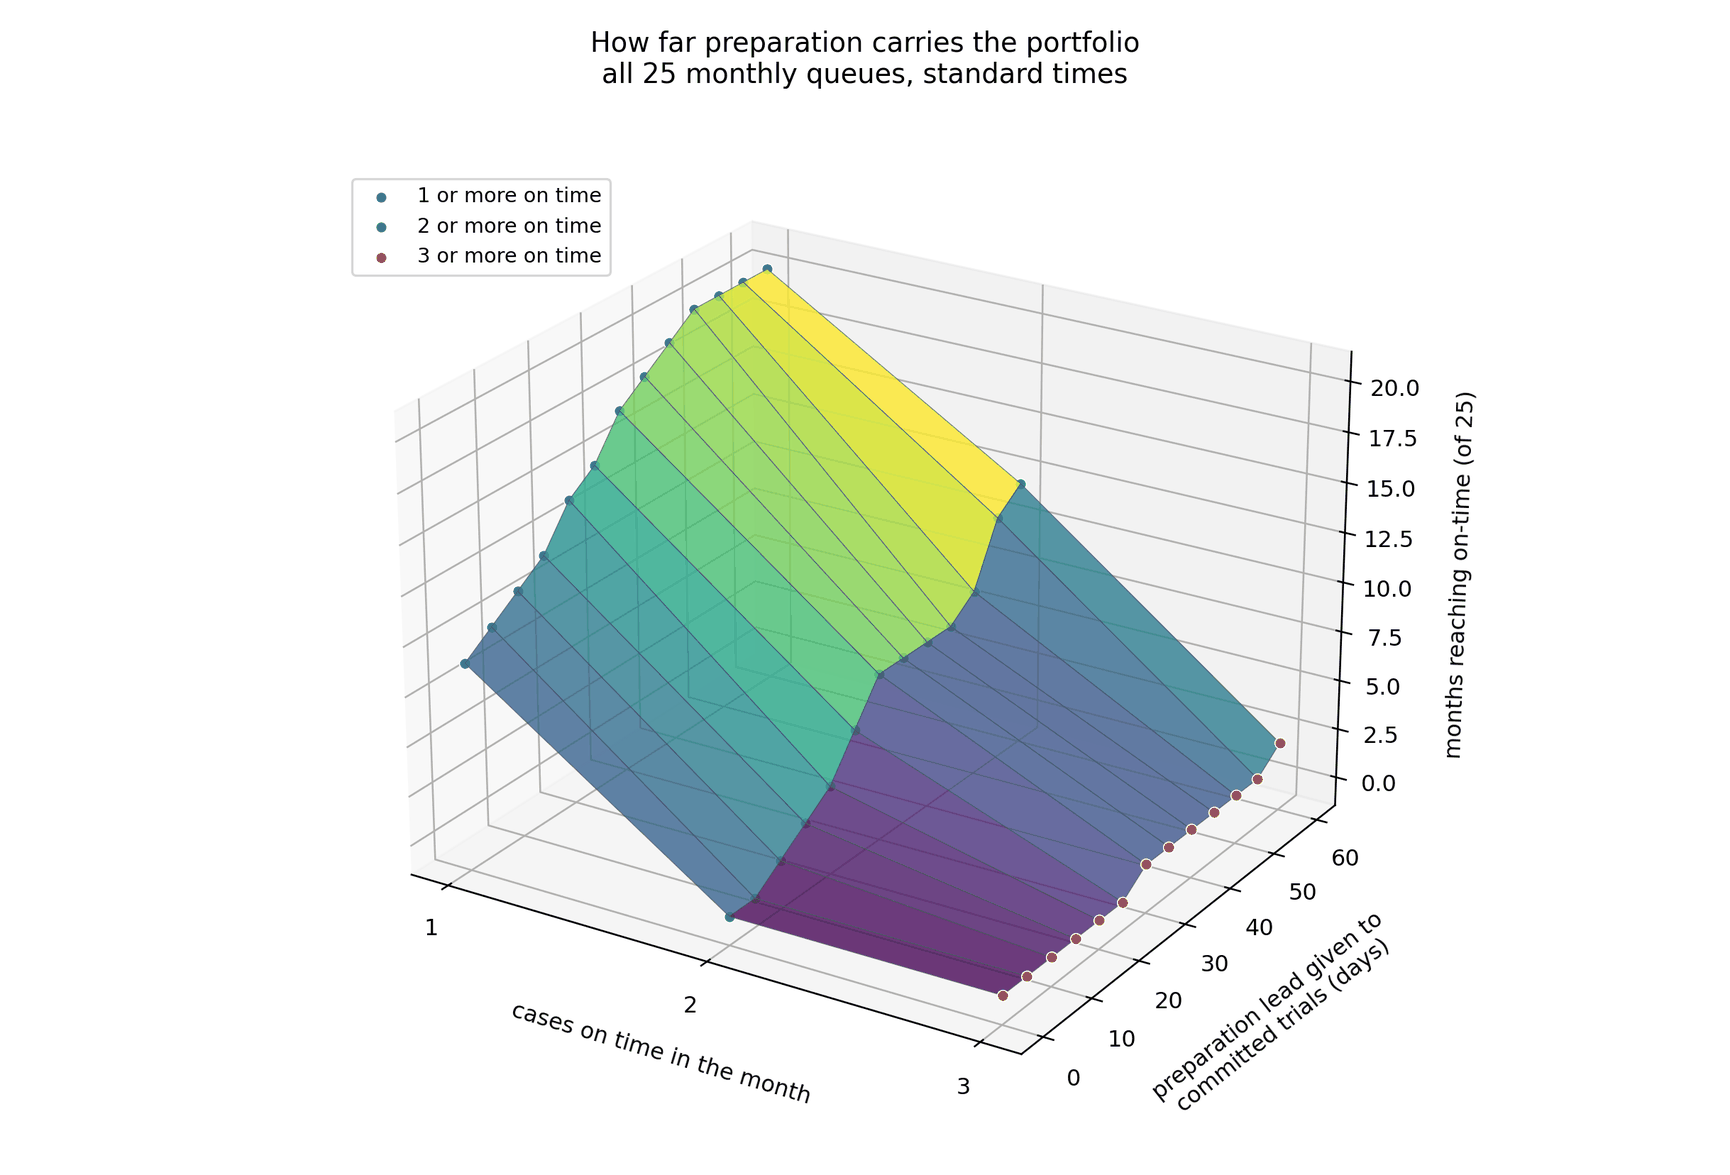
\includegraphics[width=\textwidth]{fig5_7_preparation_surface.png}
  \caption{How far preparation carries the portfolio}
  \label{fig:preparation}
\end{figure}

Approval time is the only assumption in the table without direct measurement, because the August 2026 questionnaire gave a range rather than a value. The commitment limit is a maximum, not a requirement: if opening six set-ups would create a long signature queue, the model commits fewer trials instead. Approval time therefore limits how much capacity is usable, not the on-time ceiling. Appendix 5.C reports the wait at each level and how many set-ups are worth opening.

\section{Which studies preparation should reach}
\label{sec:targeting}

Table~\ref{tab:settings} makes preparation the strongest lever; pharmacy burden says which studies should receive it.

Burden does not make set-up take longer: the work-duration distributions for the three burden bands do not differ significantly (Kruskal-Wallis $p = 0.557$). Instead, burden raises the fastest observed duration in each band: 23 days for low burden, 40 for medium burden, and 60 for high burden (Table 4.H.3). This leaves 37 days of slack within the 60-day target for low-burden trials, 20 for medium-burden trials, and none for high-burden trials.

The median time between the target clock starting and pharmacy receiving the study is 14 days (Appendix 4.D); low- and medium-burden trials can absorb this delay. High-burden trials cannot absorb even one day; Figure~\ref{fig:burdenslack} sets the three bands against the window. The exclusion is therefore structural. Of the six high-burden trials, the two that began before the clock started met the target, whereas all four that began afterwards missed it (Fisher's exact test, $p = 0.067$).

\begin{figure}[htbp]
  \centering
  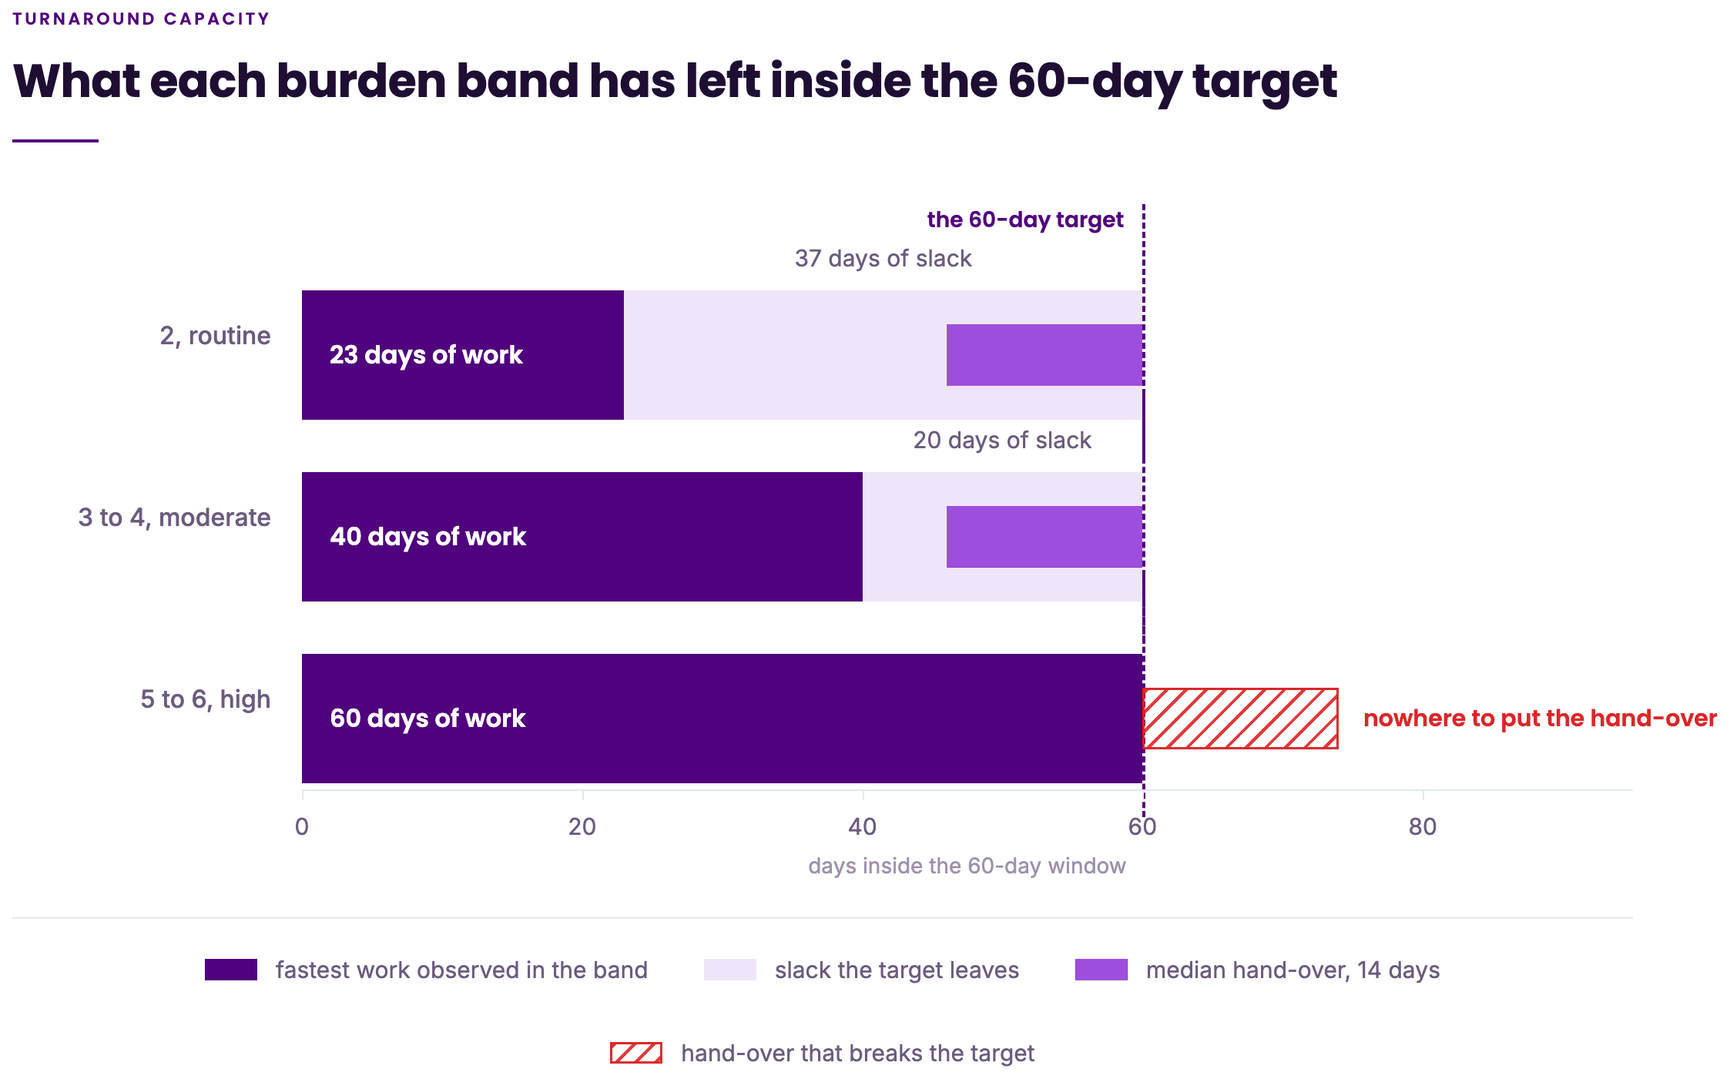
\includegraphics[width=\textwidth]{fig5_9_burden_slack.png}
  \caption{What each burden band has left inside the 60-day target}
  \label{fig:burdenslack}
\end{figure}

Preparation is the only lever these studies have, and it is not aimed at them: burden rank does not predict which trials start early (Fisher $p = 1.000$, Appendix 4.I). All six high-burden trials are aseptic, and eleven trials in the set are, so the aseptic flag identifies every one of them at notification and five others besides.

Targeting preparation at the aseptic-flagged studies concentrates effort on identifiable high-burden risk for about half the earlier notification, but its achievable on-time count is lower than preparing every committed trial, because it leaves the rescuable non-flagged trials untreated (Appendix 5.B).

The lead must be sized against the variation in durations rather than against the shortfall it closes. Appendix 5.F shows the four-day fix for BNT327-06 delivering half the time. Reading a reliability as the proportion of runs in which a plan delivers the stated outcome, a high-burden study planned at the 63-day floor is 50 per cent reliable with no lead, 75 per cent with a 28-day lead, and 90 per cent only at a 63-day lead, a second window on top of the first. Preparation is what makes a high-burden study possible; a few days of it buy a plan that says yes rather than a delivery that can be relied on.

\section{The trade-off the service faces}
\label{sec:tradeoff}

Preparation is the intervention considered here. This section reports the trade-offs it creates because the model ranks two objectives that do not always align.

The trade-off between on-time completion and weighted lateness appears only where preparation remains insufficient. On the largest queue, 1 May 2025, a 21-day lead makes each rescue cost additional lateness, whereas a 35-day lead brings two trials in on time at the lowest weighted lateness of any plan; on the 1 February 2025 queue the two objectives never conflict at any lead. Figure~\ref{fig:frontier} sets the two leads side by side and Appendix 5.C reports the frontier values.

\textbf{The conflict between finishing on time and minimising lateness is itself a symptom of insufficient preparation.} A governance rule that ranks lateness first gives up nothing when preparation is adequate and two rescues when it is not, so it is the wrong rule to fix in advance.

\begin{figure}[htbp]
  \centering
  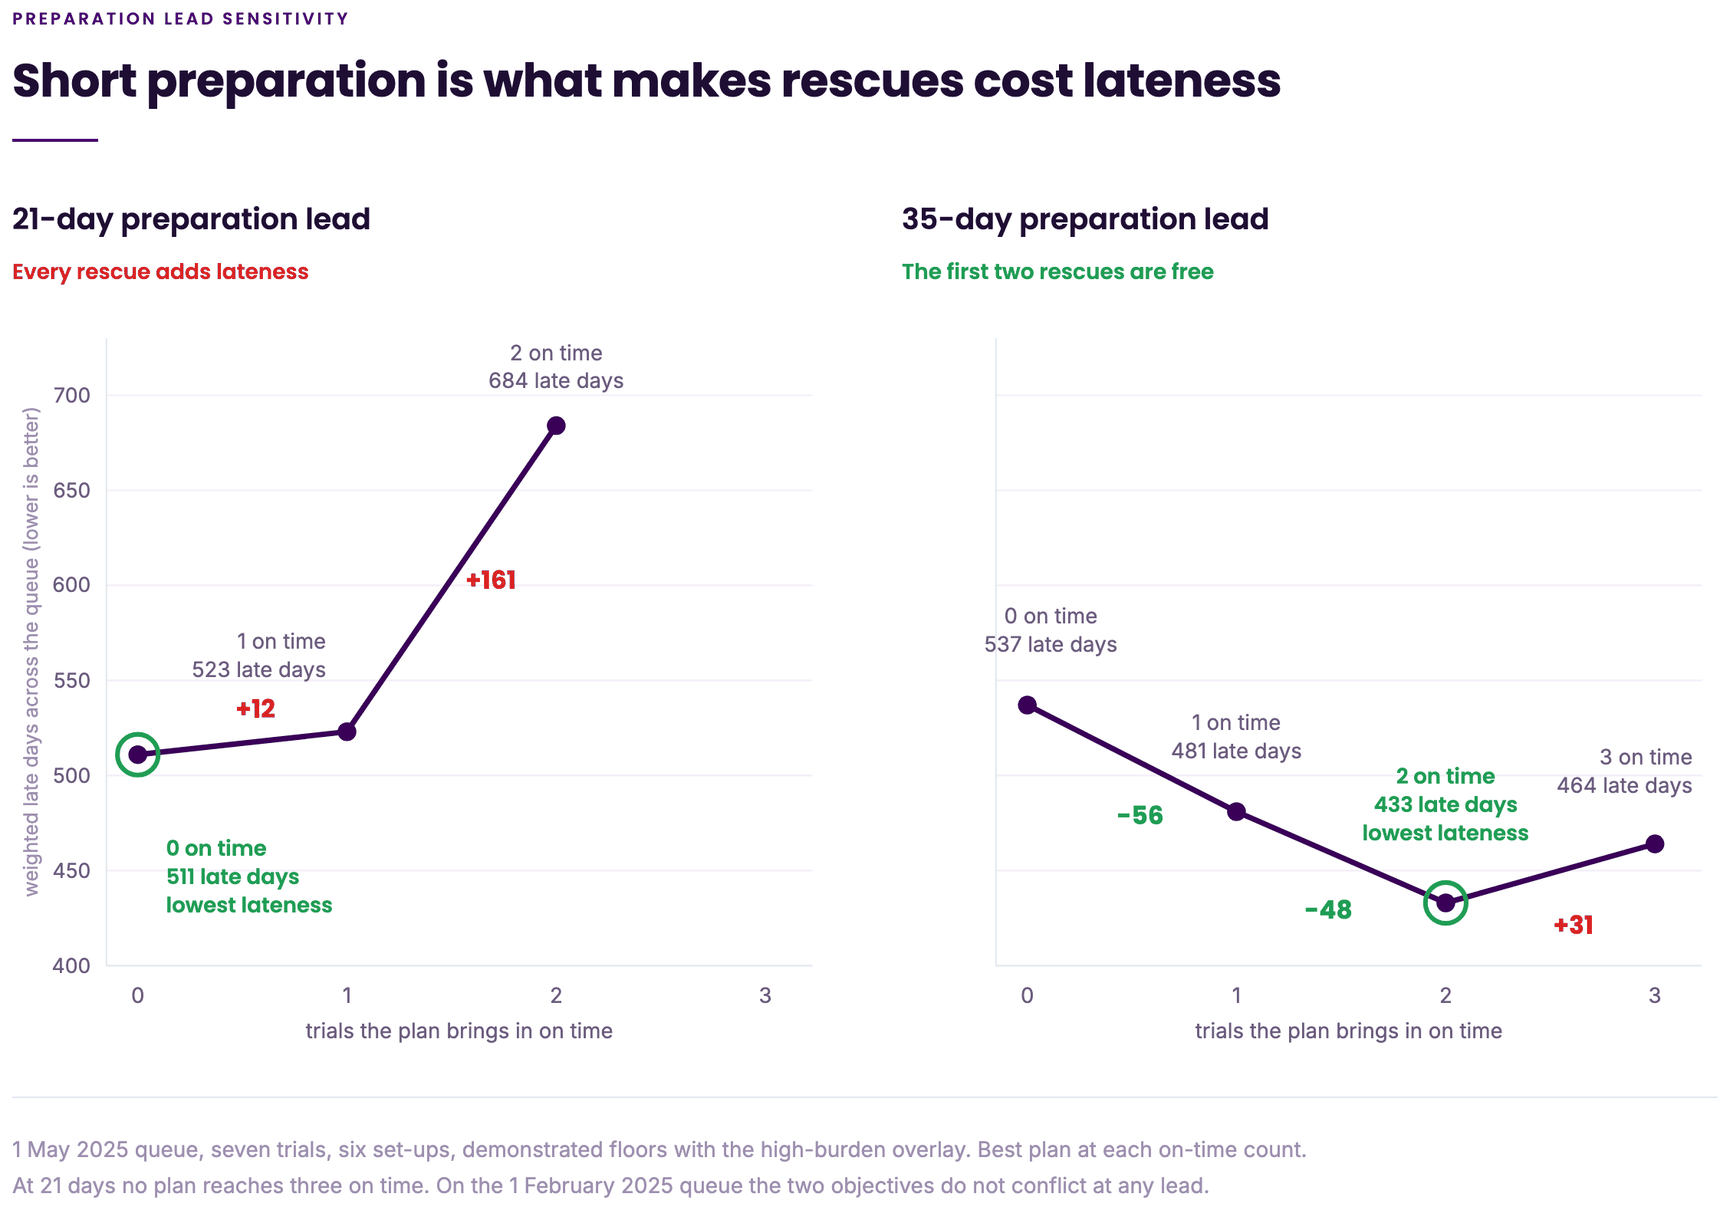
\includegraphics[width=\textwidth]{fig5_11_frontier_rotation.png}
  \caption{What a rescue costs at two preparation leads}
  \label{fig:frontier}
\end{figure}

The second trade-off is between the on-time count and the preparation it requires, the cost the trust pays in days R\&I must find. Figure~\ref{fig:prepsteps} reports the least preparation that first reaches each count.

\begin{figure}[htbp]
  \centering
  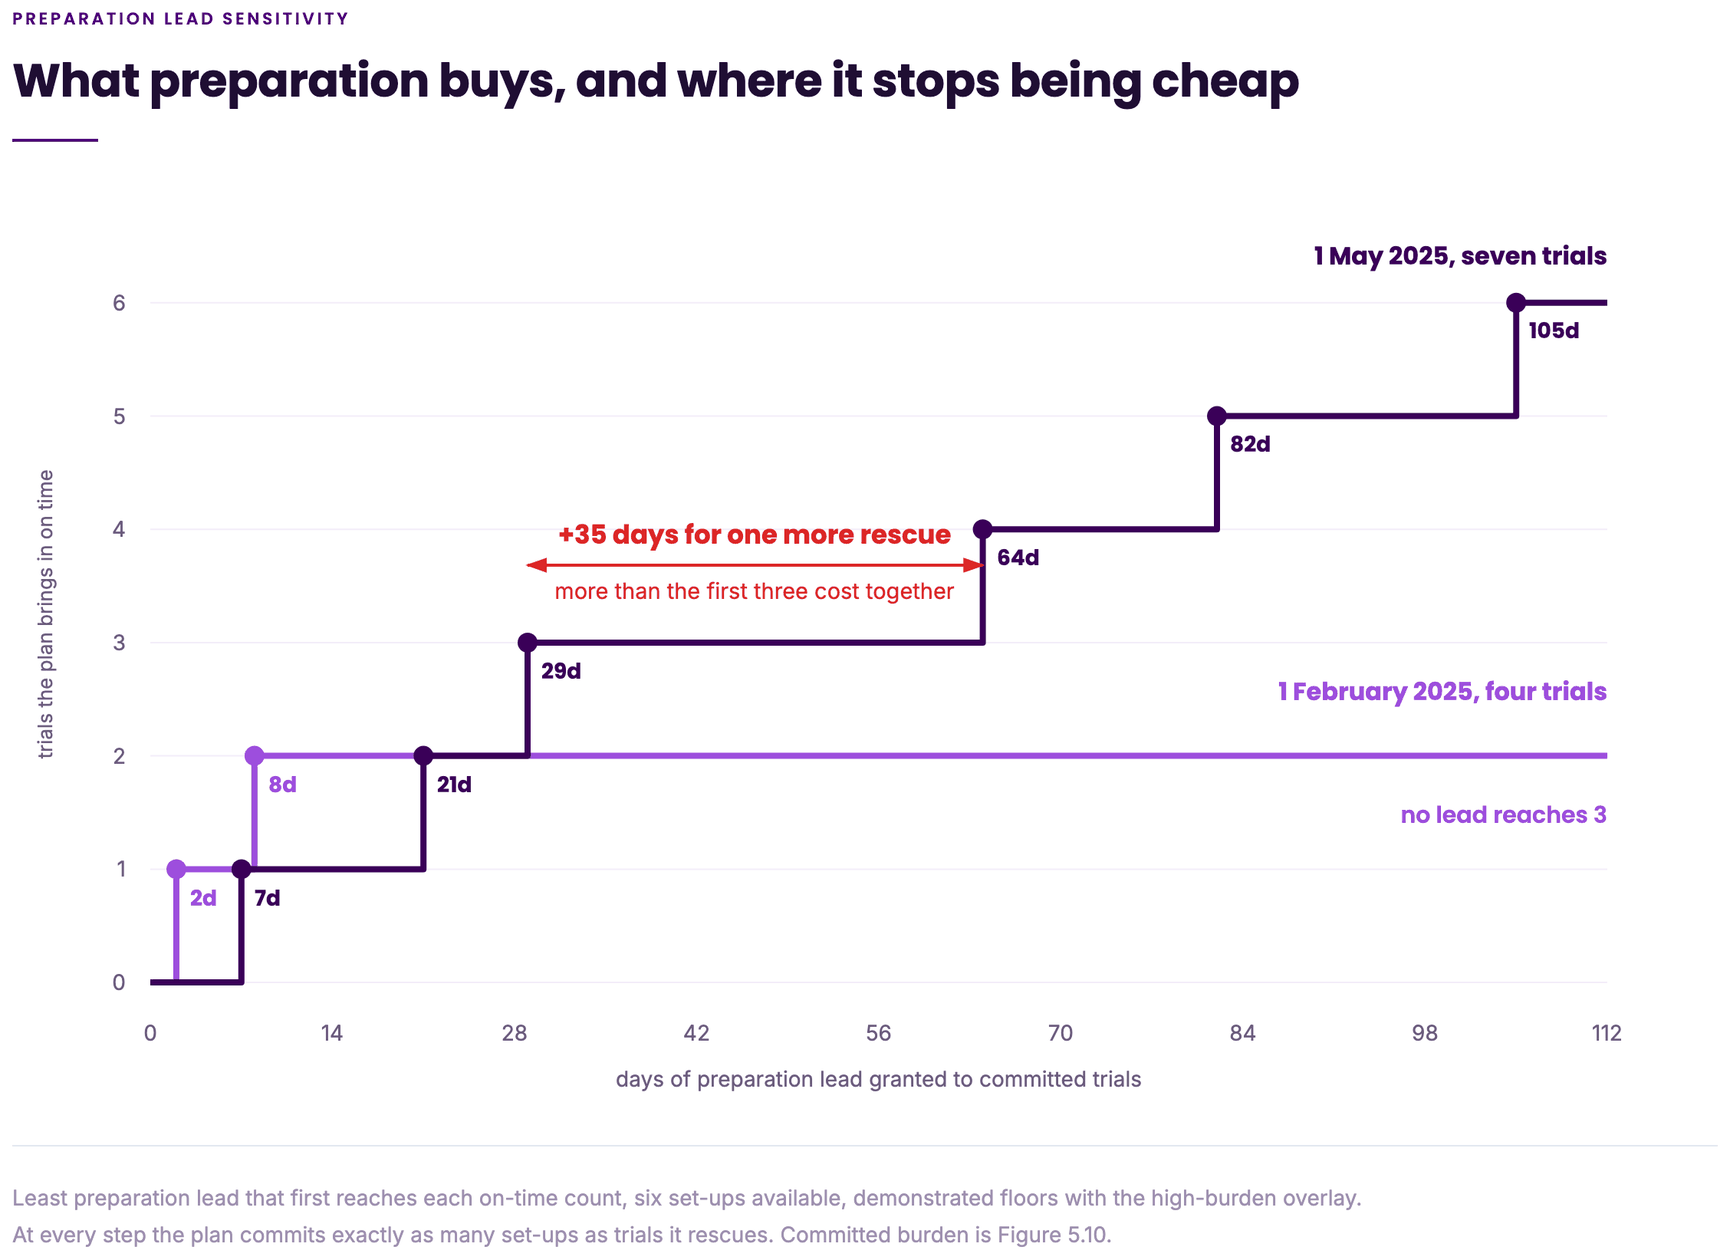
\includegraphics[width=\textwidth]{fig5_12_preparation_steps.png}
  \caption{What preparation buys, and where it stops being cheap}
  \label{fig:prepsteps}
\end{figure}

Two things follow.

First, capacity never limits the on-time count. Each rescue requires one set-up slot, so a plan that rescues three trials uses only three of the six available slots.

Second, what a queue can reach is set by its own composition. A lead only repays a shortfall the queue already carried, so it buys a rescue cheaply while a trial is near its window and buys little once a trial is far past it. Across the whole range Figure~\ref{fig:prepsteps} covers, the February queue never passes two. That ceiling belongs to the queue rather than to any lever, and it is the honest limit on what scheduling can promise.

Capacity does not stop working above the rescue count, however. Figure~\ref{fig:tradeoffpair} holds the preparation lead at 35 days and varies the set-ups opened per month against the on-time count. Lateness falls with every slot opened at each on-time count, while the pharmacy burden a plan commits rises with both. Opening more set-ups is therefore a lever on how late the rest of the queue runs rather than on how many trials meet the target. Appendix 5.C gives the values and the derived burden scale.

\begin{figure}[htbp]
  \centering
  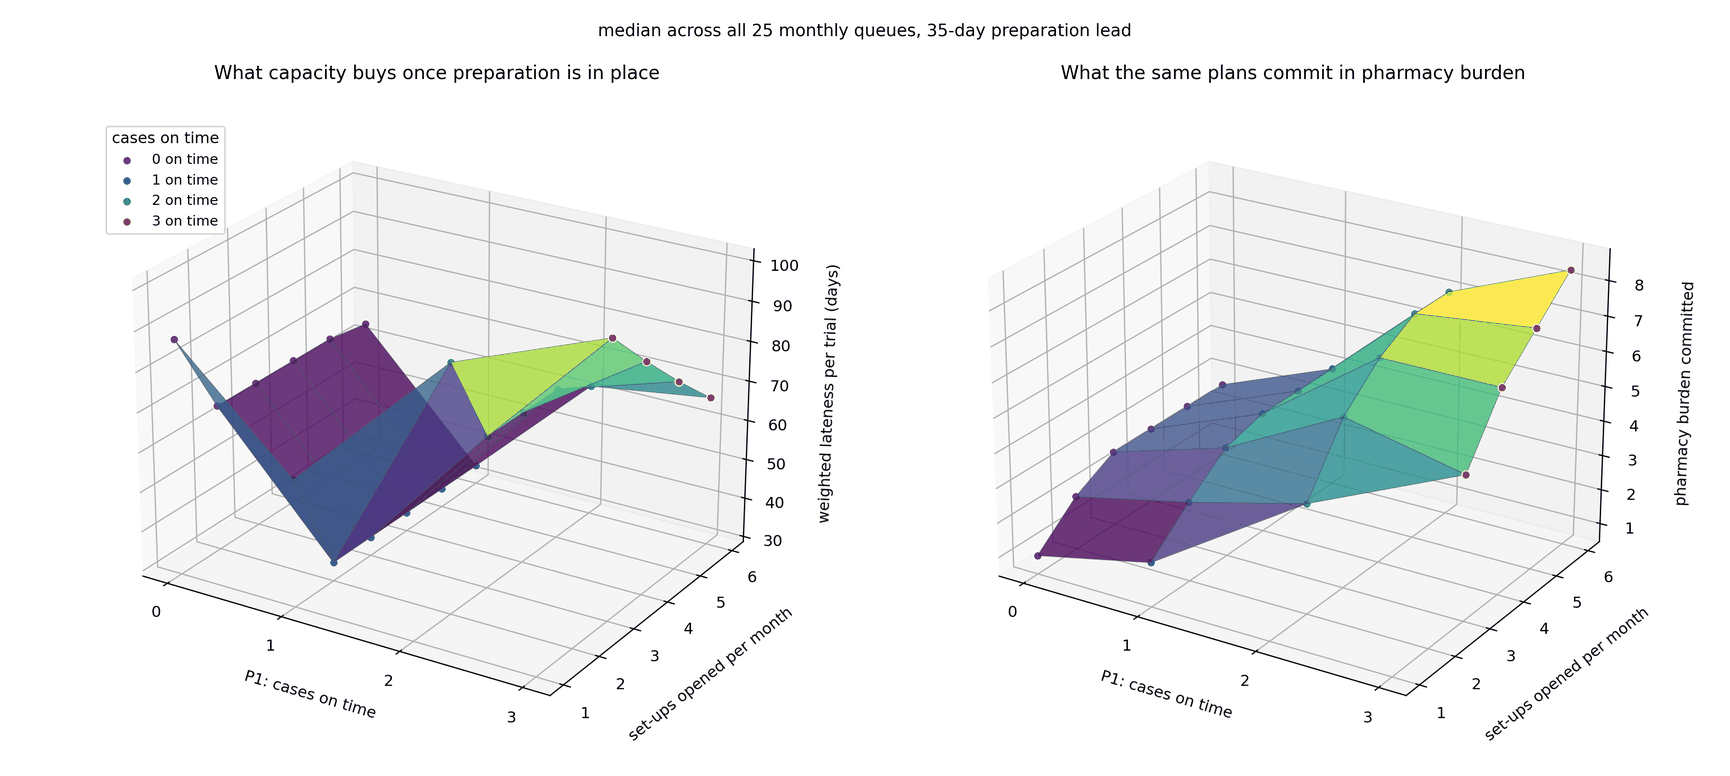
\includegraphics[width=\textwidth]{fig5_13_tradeoff_pair.png}
  \caption{What capacity buys, in days and in burden}
  \label{fig:tradeoffpair}
\end{figure}

